\chapter{Synthesis Strategy and Green Chemistry}\label{ch:g12:synthesis-strategy}

The same painkiller, ibuprofen, has been made in two ways. The older
route takes six steps, and of every hundred kilograms of starting
materials it buys, sixty end up as waste. The newer one takes three
steps, and keeps almost every \omterm{def:g7:atoms-and-molecules:atom}{atom} it buys. Both give the same white
powder in the tablet; they differ in the planning. A chemist who plans a
\omterm{def:g10:synthesis-yield:synthesis}{synthesis} asks four questions: how to go fast, how to get much, how to
touch only the right part of a \omterm{def:g7:atoms-and-molecules:molecule}{molecule}, and how to waste little.

\begin{recall}
A \omterm{def:g10:synthesis-yield:synthesis}{synthesis}: reaction, separation, purification, identification; its
\omterm{def:g10:synthesis-yield:yield}{yield} (\cref{ch:g10:synthesis-yield}). \omterm{def:g12:curly-arrows:curly-arrow}{Curly arrows}, substitution,
addition, \omterm{def:g12:curly-arrows:categories}{elimination} (\cref{ch:g12:curly-arrows}). A \omterm{def:g12:catalysis:catalyst}{catalyst} speeds up
a reaction without being consumed (\cref{ch:g12:catalysis}). A
\omterm{def:g12:equilibrium:non-total}{non-total reaction} stops at $Q = K$; an excess of a \omterm{def:g7:chemical-reactions:reactant}{reactant}, or the
removal of a product, carries it further (\cref{ch:g12:equilibrium}).
\end{recall}

\begin{omfigure}
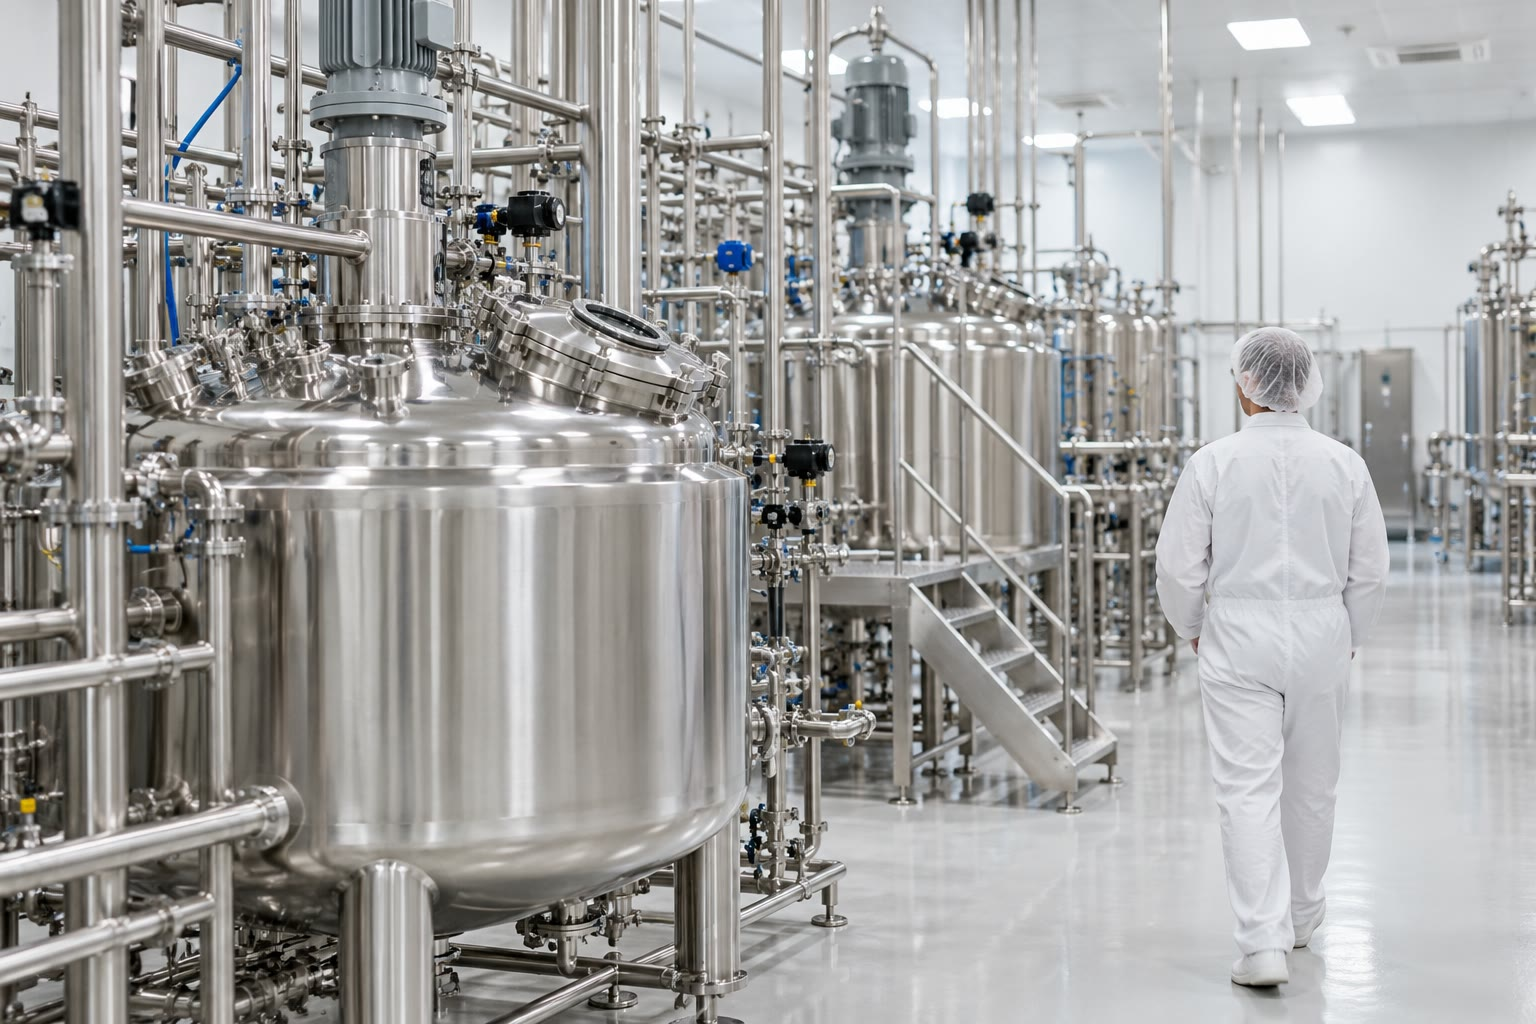
\includegraphics[width=0.48\linewidth]{images/book1/ai/g12-pharma-plant.jpg}

{\small A pharmaceutical plant: the reactors of a \omterm{def:g10:synthesis-yield:synthesis}{synthesis}, scaled up
to tonnes.}
\end{omfigure}

\section{Optimising a synthesis}

Two different things can be improved: the \emph{rate}, which decides how
long the \omterm{def:g10:synthesis-yield:synthesis}{synthesis} takes, and the \emph{\omterm{def:g10:synthesis-yield:yield}{yield}}, which decides how much
product it gives.

\begin{proposition}[Levers on rate and yield]\label{prop:g12:synthesis-strategy:levers}
\begin{itemize}
  \item The rate rises with the temperature, with the concentrations of
        the \omterm{def:g7:chemical-reactions:reactant}{reactants}, and with a \omterm{def:g12:catalysis:catalyst}{catalyst}.
  \item The final \omterm{def:g10:synthesis-yield:yield}{yield} of a \omterm{def:g10:reaction-progress-table:limiting}{total reaction} is fixed by the \omterm{def:g10:reaction-progress-table:limiting}{limiting
        reactant}; that of a \omterm{def:g12:equilibrium:non-total}{non-total reaction} rises with an excess of
        one \omterm{def:g7:chemical-reactions:reactant}{reactant}, or with the removal of a product as it forms. A
        \omterm{def:g12:catalysis:catalyst}{catalyst} does not change it: it only brings the system faster to
        the same \omterm{def:g10:reaction-progress-table:system}{final state}.
\end{itemize}
\end{proposition}

\begin{proof}
The first point gathers the \omterm{def:g12:reaction-rates:kinetic-factor}{kinetic factors} of
\cref{ch:g12:reaction-rates,ch:g12:catalysis}. The second follows from
$Q = K$ at the end of a \omterm{def:g12:equilibrium:non-total}{non-total reaction}: adding a \omterm{def:g7:chemical-reactions:reactant}{reactant} or removing
a product makes $Q < K$, and the reaction goes on forwards.
\end{proof}

\begin{example}[Esterification with a water trap]\label{ex:g12:synthesis-strategy:trap}
Ethanoic acid and ethanol, one \omterm{def:g10:the-mole:amount}{mole} of each, give only
\qty{67}{\percent} of \omterm{def:g11:functional-groups:carboxylic-acid}{ester} at equilibrium. If the \omterm{def:g6:pure-substances-and-mixtures:mixture}{mixture} is heated
under reflux in a \omterm{def:g6:solutions-and-solubility:solute}{solvent} that does not \omterm{def:g2:mixing-and-dissolving:mix}{mix} with water, with a little
acid as \omterm{def:g12:catalysis:catalyst}{catalyst}, the vapour condenses into a side tube, a \emph{water
trap}: the water, denser, settles at the bottom and stays there, while
the \omterm{def:g6:solutions-and-solubility:solute}{solvent} flows back into the flask. Water leaves the reaction as it
forms, $Q$ stays below $K$, and the esterification goes almost to
completion. The heating gives the rate, the \omterm{def:g12:catalysis:catalyst}{catalyst} more rate, the trap
the \omterm{def:g10:synthesis-yield:yield}{yield}.
\end{example}

\begin{omfigure}
\begin{tikzpicture}[font=\small, scale=0.8]
  \pic[transform shape] at (0,0) {hotplate};
  \pic[transform shape] at (0,0) {rbflask={0.55}{orange!20}};
  % the trap: water at the bottom, solvent above, up to the arm
  \fill[cyan!60!blue!40] (1.0,1.75) arc[start angle=180, end angle=360, radius=0.15] -- (1.3,2.3) -- (1.0,2.3) -- cycle;
  \fill[yellow!35] (1.0,2.3) rectangle (1.3,3.25);
  \draw[om glass] (-0.2,3.0) -- (-0.2,3.75) -- (0.2,3.75) -- (0.2,3.55) -- (1.0,3.55) -- (1.0,4.0);
  \draw[om glass] (0.2,3.0) -- (0.2,3.25) -- (1.0,3.25) -- (1.0,1.75) arc[start angle=180, end angle=360, radius=0.15] -- (1.3,4.0);
  \pic[transform shape] at (1.15,4.0) {condenser};
  \draw[omProp, thick, <-] (1.35,2.0) -- (2.6,1.7) node[right, text=black, align=left] {water collects\\ at the bottom};
  \draw[omProp, thick, <-] (1.35,2.9) -- (2.6,3.1) node[right, text=black, align=left] {the solvent overflows\\ back to the flask};
  \draw[omProp, thick, <-] (-0.6,0.6) -- (-1.7,1.1) node[left, text=black, align=right] {acid, alcohol,\\ catalyst, solvent};
\end{tikzpicture}

{\small A water trap on a flask heated under reflux: the water formed is
removed from the reaction as it condenses.}
\end{omfigure}

\section{Selectivity}

A real \omterm{def:g7:atoms-and-molecules:molecule}{molecule} often carries several \omterm{def:g11:functional-groups:functional-group}{functional groups}. A \omterm{def:g7:identifying-substances:characteristic-test}{reagent} that
attacks them all gives a \omterm{def:g6:pure-substances-and-mixtures:mixture}{mixture}; a good \omterm{def:g10:synthesis-yield:synthesis}{synthesis} uses one that attacks
only the group to be changed.

\begin{definition}[Chemoselective reaction]\label{def:g12:synthesis-strategy:chemoselective}
A reaction is \emph{chemoselective}\index{chemoselective reaction} when,
on a \omterm{def:g7:atoms-and-molecules:molecule}{molecule} carrying several \omterm{def:g11:functional-groups:functional-group}{functional groups}, its \omterm{def:g7:identifying-substances:characteristic-test}{reagent} transforms
one group and leaves the others unchanged.
\end{definition}

\begin{example}[A reductant that chooses]\label{ex:g12:synthesis-strategy:nabh4}
Sodium borohydride, \ce{NaBH4}, reduces the carbonyl group of \omterm{def:g11:functional-groups:carbonyl}{aldehydes}
and \omterm{def:g11:functional-groups:carbonyl}{ketones} into an \omterm{def:g11:functional-groups:alcohol}{alcohol} group, but leaves \omterm{def:g11:functional-groups:carboxylic-acid}{esters} untouched. On a
\omterm{def:g7:atoms-and-molecules:molecule}{molecule} that carries a \omterm{def:g11:functional-groups:carbonyl}{ketone} and an \omterm{def:g11:functional-groups:carboxylic-acid}{ester}, only the \omterm{def:g11:functional-groups:carbonyl}{ketone} changes:
\[
  \ce{CH3-CO-CH2-CH2-CO-O-CH3}
  \;\xrightarrow{\ \ce{NaBH4}\ }\;
  \ce{CH3-CH(OH)-CH2-CH2-CO-O-CH3} .
\]
A stronger \omterm{def:g11:redox:oxidant}{reductant}, lithium aluminium hydride \ce{LiAlH4}, would reduce
both groups: it is not \omterm{def:g12:synthesis-strategy:chemoselective}{chemoselective} here.
\end{example}

\begin{remark}[Several kinds of selectivity]\label{rem:g12:synthesis-strategy:kinds}
Chemoselectivity chooses between groups. A reaction can also choose
between two positions of the same group, or between two \omterm{def:g12:stereochemistry:stereoisomer}{stereoisomers} of
the product, as the \omterm{def:g12:catalysis:enzyme}{enzymes} of \cref{ch:g12:catalysis} and the \omterm{def:g12:stereochemistry:chiral}{chiral}
\omterm{def:g7:atoms-and-molecules:molecule}{molecules} of \cref{ch:g12:stereochemistry} showed. Each kind is studied
in the university volumes.
\end{remark}

\section{Protecting groups}

When no \omterm{def:g7:identifying-substances:characteristic-test}{reagent} is selective enough, the chemist hides the group that
must not react, does the reaction, and then uncovers the group again.

\begin{definition}[Protecting group]\label{def:g12:synthesis-strategy:protecting-group}
A \emph{protecting group}\index{protecting group} is a group attached to a
\omterm{def:g11:functional-groups:functional-group}{functional group} to stop it from reacting during one or more steps of a
\omterm{def:g10:synthesis-yield:synthesis}{synthesis}, and removed afterwards to give back the original group. The
three operations are \emph{protection}, \emph{reaction} and
\emph{deprotection}.
\end{definition}

\begin{method}[Planning a protection]\label{met:g12:synthesis-strategy:plan}
\begin{enumerate}
  \item List the groups of each \omterm{def:g7:chemical-reactions:reactant}{reactant}, and the one bond to be made.
  \item Mark every other group that the \omterm{def:g7:identifying-substances:characteristic-test}{reagent} of that step could also
        attack.
  \item Protect each of them with a group that resists the reaction
        conditions and that can be removed under gentle conditions that
        leave the new bond intact.
  \item Count the cost: each protection adds two steps, protection and
        deprotection, and lowers the overall \omterm{def:g10:synthesis-yield:yield}{yield}.
\end{enumerate}
\end{method}

\begin{example}[Making one dipeptide, not four]\label{ex:g12:synthesis-strategy:dipeptide}
Glycine, \ce{H2N-CH2-COOH}, and alanine, \ce{H2N-CH(CH3)-COOH}, each carry
an \omterm{def:g11:functional-groups:amine}{amine} group and an acid group. An \omterm{def:g11:functional-groups:amine}{amide} bond between the acid of
glycine and the \omterm{def:g11:functional-groups:amine}{amine} of alanine gives the dipeptide Gly--Ala. Mixed
directly, the two amino acids give four dipeptides, Gly--Ala, Ala--Gly,
Gly--Gly and Ala--Ala, in a \omterm{def:g6:pure-substances-and-mixtures:mixture}{mixture} hard to separate. The plan:
\begin{enumerate}
  \item protect the \omterm{def:g11:functional-groups:amine}{amine} of glycine with a group written \ce{Z}, and the
        acid of alanine as its methyl \omterm{def:g11:functional-groups:carboxylic-acid}{ester};
  \item form the \omterm{def:g11:functional-groups:amine}{amide} bond: only one acid group and one \omterm{def:g11:functional-groups:amine}{amine} group are
        left free;
  \item remove both \omterm{def:g12:synthesis-strategy:protecting-group}{protecting groups}.
\end{enumerate}
\end{example}

\begin{omfigure}
\begin{tikzpicture}[font=\small, node distance=0.55cm,
    box/.style={draw=omDef, rounded corners=2pt, fill=omDef!6, align=center, inner sep=4pt}]
  \node[box] (a) {\ce{H2N-CH2-COOH}\\ \ce{H2N-CH(CH3)-COOH}};
  \node[box, below=of a] (b) {\ce{Z-NH-CH2-COOH}\\ \ce{H2N-CH(CH3)-CO-O-CH3}};
  \node[box, below=of b] (c) {\ce{Z-NH-CH2-CO-NH-CH(CH3)-CO-O-CH3}};
  \node[box, below=of c] (d) {\ce{H2N-CH2-CO-NH-CH(CH3)-COOH}};
  \draw[->, thick, omProp] (a) -- node[right, xshift=3pt, text=black] {1. protection} (b);
  \draw[->, thick, omProp] (b) -- node[right, xshift=3pt, text=black] {2. reaction: amide bond} (c);
  \draw[->, thick, omProp] (c) -- node[right, xshift=3pt, text=black] {3. deprotection} (d);
  \node[anchor=east, font=\footnotesize, text=black!70] at ([xshift=-6pt]a.west) {glycine, alanine};
  \node[anchor=east, font=\footnotesize, text=black!70] at ([xshift=-6pt]d.west) {Gly--Ala};
\end{tikzpicture}

{\small Protection, reaction, deprotection: the only \omterm{def:g11:functional-groups:amine}{amide} bond that can
form is the one wanted.}
\end{omfigure}

\section{Atom economy}

A \omterm{def:g10:synthesis-yield:yield}{yield} of \qty{100}{\percent} says that every \omterm{def:g7:atoms-and-molecules:molecule}{molecule} of the \omterm{def:g10:reaction-progress-table:limiting}{limiting
reactant} became product. It does not say how many of the \omterm{def:g7:atoms-and-molecules:atom}{atoms} bought
ended up in the product: the other products of the equation, however
pure, are waste unless someone can use them.

\begin{definition}[Atom economy]\label{def:g12:synthesis-strategy:atom-economy}
The \emph{atom economy}\index{atom economy} of a \omterm{def:g10:synthesis-yield:synthesis}{synthesis} is the
fraction of the mass of the \omterm{def:g7:chemical-reactions:reactant}{reactants}, taken in the proportions of the
\omterm{def:g8:balanced-equations:equation}{balanced equation}, that ends up in the desired product.
\end{definition}

\begin{proposition}[Atom economy from the equation]\label{prop:g12:synthesis-strategy:atom-economy}
For a \omterm{def:g8:balanced-equations:equation}{balanced equation} $a_1\,\ce{R1} + a_2\,\ce{R2} + \cdots \rightarrow
p\,\ce{P} + \text{other products}$,
\[
  \text{atom economy} =
  \frac{p\,M(\ce{P})}{a_1 M(\ce{R1}) + a_2 M(\ce{R2}) + \cdots}
  \times 100\,\% .
\]
\end{proposition}

\begin{proof}
For $x$ \omterm{def:g10:the-mole:amount}{moles} of reaction, the mass of \omterm{def:g7:chemical-reactions:reactant}{reactants} consumed is
$x\,(a_1 M(\ce{R1}) + \cdots)$ and the mass of desired product formed is
$x\,p\,M(\ce{P})$; their ratio does not depend on $x$.
\end{proof}

\begin{method}[Computing an atom economy]\label{met:g12:synthesis-strategy:atom-economy}
\begin{enumerate}
  \item Write the \omterm{def:g8:balanced-equations:equation}{balanced equation}; for a route of several steps, add the
        steps so that every intermediate cancels.
  \item Compute the \omterm{def:g10:the-mole:molar-mass}{molar mass} of each \omterm{def:g7:chemical-reactions:reactant}{reactant} and of the desired
        product.
  \item Apply the formula, with the \omterm{def:g8:balanced-equations:coefficient}{stoichiometric coefficients}.
  \item The waste per kilogram of product is
        $(100 - \text{atom economy})/\text{atom economy}$ kilograms.
\end{enumerate}
\end{method}

\begin{example}[Addition against substitution]\label{ex:g12:synthesis-strategy:compare}
% ledger: aw:C, aw:H, aw:Br, aw:Na, aw:O
Bromoethane from ethene, \ce{C2H4 + HBr -> C2H5Br}: every \omterm{def:g7:atoms-and-molecules:atom}{atom} ends up
in the product, \omterm{def:g12:synthesis-strategy:atom-economy}{atom economy} $108.9/(28.0 + 80.9) = \qty{100}{\percent}$.
Ethanol from bromoethane, \ce{C2H5Br + NaOH -> C2H5OH + NaBr}: the
\omterm{def:g12:synthesis-strategy:atom-economy}{atom economy} is $46.0/(108.9 + 40.0) = \qty{30.9}{\percent}$; per
kilogram of ethanol, \qty{2.2}{kg} of sodium bromide. An addition always
has an \omterm{def:g12:synthesis-strategy:atom-economy}{atom economy} of \qty{100}{\percent}; a substitution or an
\omterm{def:g12:curly-arrows:categories}{elimination} never does.
\end{example}

\begin{omfigure}
\begin{tikzpicture}
\begin{axis}[width=0.8\linewidth, height=5.2cm, ybar, bar width=16pt,
    ymin=0, ymax=112, ylabel={atom economy (\%)},
    xtick={1,2,3,4,5}, xticklabels={addition, esterification, ibuprofen (3 steps), ibuprofen (6 steps), substitution},
    xticklabel style={font=\footnotesize, align=center, text width=2.1cm},
    nodes near coords, nodes near coords style={font=\footnotesize},
    enlarge x limits=0.12, axis lines*=left, ymajorgrids, grid style={black!12}]
  \addplot[fill=omDef!55, draw=omDef] table[x=i, y=AE] {figdata/out/grade-12-synthesis-strategy.dat};
\end{axis}
\end{tikzpicture}

{\small \omterm{def:g7:atoms-and-molecules:atom}{Atom} economies computed from the equations: ethene with hydrogen
bromide, ethanoic acid with ethanol, the two ibuprofen routes, and
bromoethane with sodium hydroxide.}
\end{omfigure}

\section{Green chemistry}

\begin{definition}[Green chemistry]\label{def:g12:synthesis-strategy:green-chemistry}
\emph{Green chemistry}\index{green chemistry} is the design of chemical
products and processes that reduce or eliminate the use and the
production of hazardous substances, from the choice of the starting
materials to the fate of the product after use.
\end{definition}

Twelve principles summarise the approach; each is a question to ask of a
process.
% ledger: green:12
\begin{enumerate}
  \item Prevent waste rather than treat it.
  \item Maximise \omterm{def:g12:synthesis-strategy:atom-economy}{atom economy}.
  \item Design less hazardous syntheses.
  \item Design safer chemicals and products.
  \item Use safer \omterm{def:g6:solutions-and-solubility:solute}{solvents} and reaction conditions.
  \item Increase energy efficiency: work near room temperature and
        pressure.
  \item Use renewable feedstocks.
  \item Avoid chemical derivatives, such as \omterm{def:g12:synthesis-strategy:protecting-group}{protecting groups}.
  \item Use \omterm{def:g12:catalysis:catalyst}{catalysts}, not stoichiometric \omterm{def:g7:identifying-substances:characteristic-test}{reagents}.
  \item Design products that degrade after use.
  \item Analyse in real time to prevent pollution.
  \item Minimise the potential for accidents.
\end{enumerate}

\begin{remark}[Principles, not laws]\label{rem:g12:synthesis-strategy:principles}
The principles often pull in opposite directions: a \omterm{def:g12:synthesis-strategy:protecting-group}{protecting group}
breaks principle 8 but may save a whole \omterm{def:g10:synthesis-yield:synthesis}{synthesis}; a \omterm{def:g12:catalysis:catalyst}{catalyst} that saves
energy may contain a scarce \omterm{def:g9:periodic-table-first-look:metal}{metal}. Judging a process means weighing them,
with numbers wherever possible: \omterm{def:g12:synthesis-strategy:atom-economy}{atom economy}, \omterm{def:g10:synthesis-yield:yield}{yield}, mass of waste,
energy.
\end{remark}

\begin{history}[Green chemistry, 1998]
% ledger: green:book-1998, ibu:bhc-commercial
In 1998 the chemists Paul Anastas and John Warner published a book,
\emph{Green Chemistry: Theory and Practice}, which laid out the twelve
principles. A year earlier, a government prize for greener syntheses had
gone to the three-step route to ibuprofen, run on an industrial scale
since 1992. Since then, the principles have been taught to chemists as
part of their trade.
\end{history}

\begin{example}[Two routes to ibuprofen]\label{ex:g12:synthesis-strategy:ibuprofen}
% ledger: ibu:boots-steps, ibu:bhc-steps, ibu:boots-ae, ibu:bhc-ae, ibu:bhc-ae-recovered
Ibuprofen, \ce{C13H18O2}, is made from the hydrocarbon
\ce{C10H14} (isobutylbenzene). The older route uses six steps and,
in each, a full amount of \omterm{def:g7:identifying-substances:characteristic-test}{reagent}; added together, its \omterm{def:g7:chemical-reactions:reactant}{reactants} have a
\omterm{def:g10:the-mole:molar-mass}{molar mass} sum of \qty{514.5}{g/mol}, for \qty{206.0}{g/mol} of
ibuprofen: \omterm{def:g12:synthesis-strategy:atom-economy}{atom economy} \qty{40}{\percent}. The newer route uses three
steps, two of them catalysed, and the overall equation
\[
  \ce{C10H14 + C4H6O3 + H2 + CO -> C13H18O2 + C2H4O2}
\]
gives $206.0/266.0 = \qty{77}{\percent}$. Its by-product, ethanoic acid,
is recovered and used: counted as a product, the \omterm{def:g12:synthesis-strategy:atom-economy}{atom economy} exceeds
\qty{99}{\percent}.
\end{example}

\begin{omfigure}
\chemfig{[:30]*6(-=(-[:90](-[:150])-[:30](=[:90]O)-[:-30]OH)-=-(-[:-90]-[:-150](-[:150])-[:-90])=)}

\medskip
\begin{tikzpicture}[font=\scriptsize,
    st/.style={draw=omDef, rounded corners=2pt, fill=omDef!6, minimum height=0.8cm, text width=1.15cm, align=center, inner sep=2pt}]
  \foreach \i/\t in {1/acylation, 2/+ 2 carbons, 3/aldehyde, 4/oxime, 5/nitrile, 6/acid}
    \node[st] (o\i) at (1.7*\i,0) {\t};
  \foreach \i/\j in {1/2,2/3,3/4,4/5,5/6} \draw[->, thick] (o\i) -- (o\j);
  \node[anchor=east, align=right, font=\footnotesize] at ([xshift=-4pt]o1.west) {6 steps\\ \textbf{40 \%}};
  \foreach \i/\t in {1/acylation, 2/adds \ce{H2}, 3/adds \ce{CO}}
    \node[st, fill=omProp!8, draw=omProp] (n\i) at (1.7*\i,-1.4) {\t\\ (catalyst)};
  \foreach \i/\j in {1/2,2/3} \draw[->, thick] (n\i) -- (n\j);
  \node[anchor=east, align=right, font=\footnotesize] at ([xshift=-4pt]n1.west) {3 steps\\ \textbf{77 \%}};
  \node[anchor=west, align=left, font=\footnotesize] at ([xshift=6pt]n3.east) {by-product: ethanoic acid, recovered;\\ counted as a product: over 99 \%};
\end{tikzpicture}

{\small Ibuprofen (top) and its two industrial routes: the older one,
six steps, and the newer one, three catalysed steps, with their \omterm{def:g7:atoms-and-molecules:atom}{atom}
economies.}
\end{omfigure}

\begin{example}[Greener solvents]\label{ex:g12:synthesis-strategy:solvents}
% ledger: crit:CO2-T, crit:CO2-p
Many reactions and \omterm{def:g10:chemical-species:extraction}{extractions} use organic \omterm{def:g6:solutions-and-solubility:solute}{solvents} that are toxic,
flammable or volatile. Water is the safest \omterm{def:g6:solutions-and-solubility:solute}{solvent} of all, when the
\omterm{def:g7:chemical-reactions:reactant}{reactants} \omterm{def:g2:mixing-and-dissolving:dissolve}{dissolve} in it. Carbon dioxide becomes another: above
\qty{31}{\celsius} and \qty{73.8}{bar} it is a \emph{supercritical
fluid}, neither liquid nor gas, which \omterm{def:g2:mixing-and-dissolving:dissolve}{dissolves} many organic \omterm{def:g7:atoms-and-molecules:molecule}{molecules}.
It extracts caffeine from coffee beans, for example; when the pressure is
released, it simply turns back into a gas and leaves no residue in the
product.
\end{example}

\begin{omfigure}
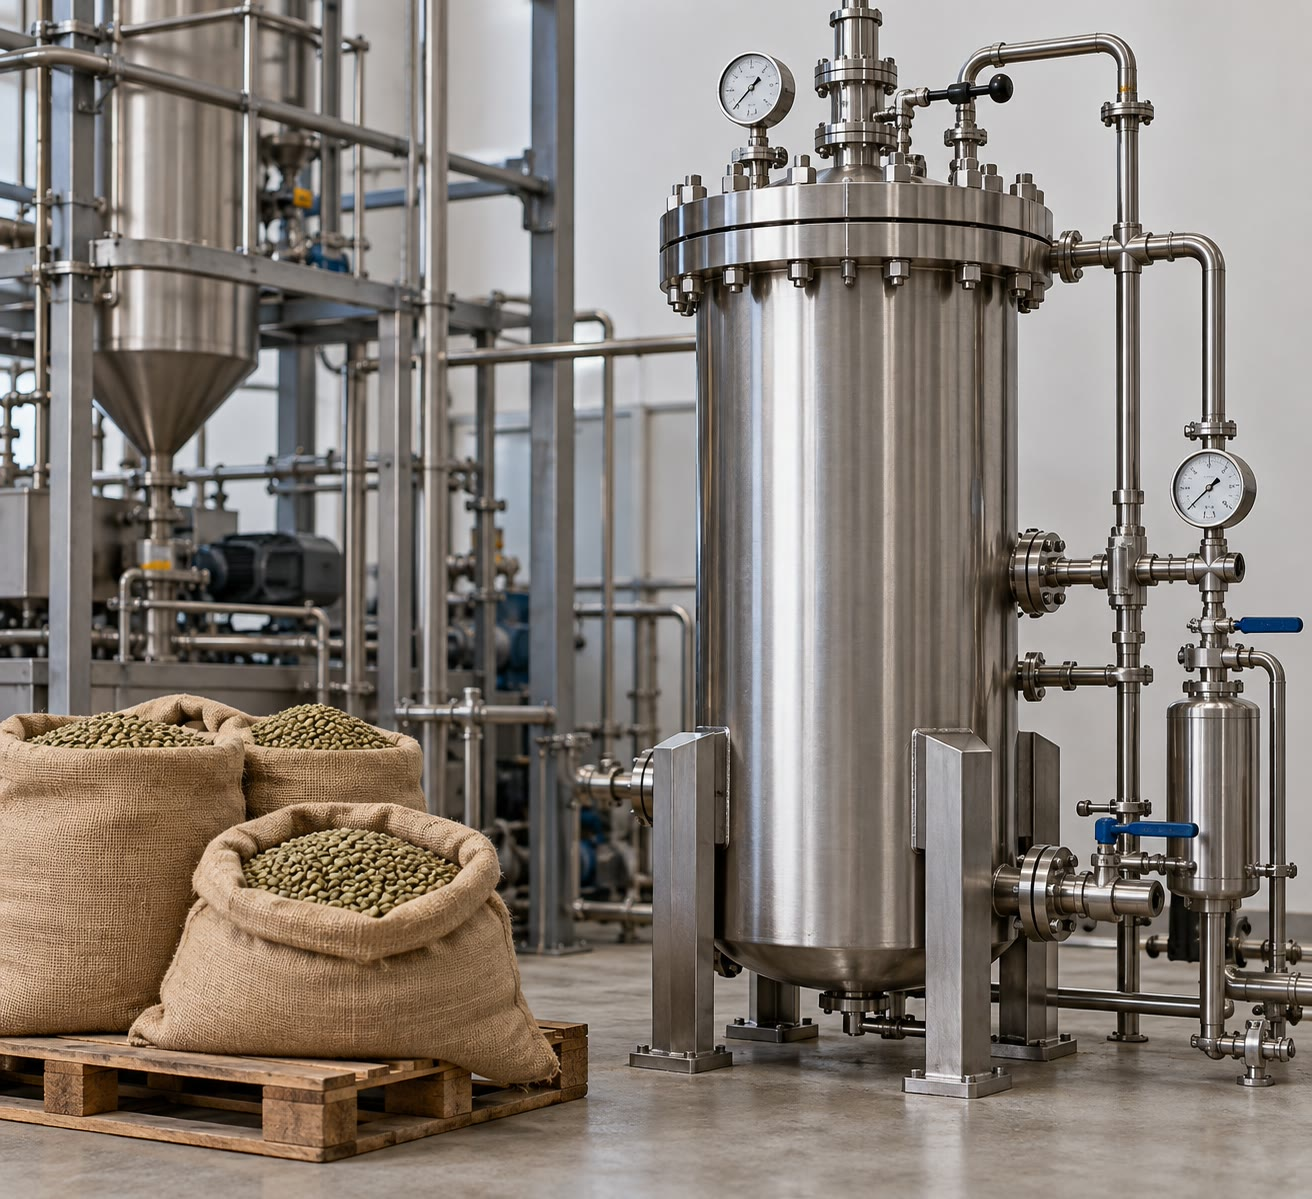
\includegraphics[width=0.45\linewidth,height=6cm,keepaspectratio]{images/book1/ai/g12-scco2-vessel.jpg}

{\small A high-pressure \omterm{def:g10:chemical-species:extraction}{extraction} vessel, in which supercritical carbon
dioxide replaces an organic \omterm{def:g6:solutions-and-solubility:solute}{solvent}.}
\end{omfigure}

\section{Exercises}

\begin{exercise}[$\star$]\label{exo:g12:synthesis-strategy:1}
Ethanol can be made by hydration of ethene, \ce{C2H4 + H2O -> C2H5OH},
or by fermentation of glucose, \ce{C6H12O6 -> 2C2H5OH + 2CO2}. Compute
the \omterm{def:g12:synthesis-strategy:atom-economy}{atom economy} of each.
\end{exercise}

\begin{exercise}[$\star$]\label{exo:g12:synthesis-strategy:2}
In the dipeptide scheme of this chapter, name the step at which each
\omterm{def:g12:synthesis-strategy:protecting-group}{protecting group} is put on, and the step at which it is taken off.
\end{exercise}

\begin{exercise}[$\star$]\label{exo:g12:synthesis-strategy:3}
A factory replaces a chlorinated \omterm{def:g6:solutions-and-solubility:solute}{solvent} by water in one of its
reactions. Which principle of \omterm{def:g12:synthesis-strategy:green-chemistry}{green chemistry} does it apply?
\end{exercise}

\begin{exercise}[$\star$]\label{exo:g12:synthesis-strategy:4}
Why does an excess of ethanol raise the \omterm{def:g10:synthesis-yield:yield}{yield} of an esterification, but
a \omterm{def:g12:catalysis:catalyst}{catalyst} does not?
\end{exercise}

\begin{exercise}[$\star$]\label{exo:g12:synthesis-strategy:5}
Sodium borohydride reduces \omterm{def:g11:functional-groups:carbonyl}{aldehydes} and \omterm{def:g11:functional-groups:carbonyl}{ketones}, not \omterm{def:g11:functional-groups:carboxylic-acid}{esters}. Is its
reaction with methyl 4-oxopentanoate (a \omterm{def:g11:functional-groups:carbonyl}{ketone} and an \omterm{def:g11:functional-groups:carboxylic-acid}{ester})
\omterm{def:g12:synthesis-strategy:chemoselective}{chemoselective}? Which group changes?
\end{exercise}

\begin{exercise}[$\star\star$]\label{exo:g12:synthesis-strategy:6}
One \omterm{def:g10:the-mole:amount}{mole} of ethanoic acid and one of ethanol give \qty{0.67}{mol} of
\omterm{def:g11:functional-groups:carboxylic-acid}{ester} at equilibrium. Propose two ways to raise this amount, and one way
to reach it faster.
\end{exercise}

\begin{exercise}[$\star\star$]\label{exo:g12:synthesis-strategy:7}
Methyl 4-oxopentanoate, \ce{CH3-CO-CH2-CH2-CO-O-CH3}, is treated once
with sodium borohydride, once with an excess of lithium aluminium
hydride, which reduces the \omterm{def:g11:functional-groups:carboxylic-acid}{ester} into two \omterm{def:g11:functional-groups:alcohol}{alcohols}. Write each product.
\end{exercise}

\begin{exercise}[$\star\star$]\label{exo:g12:synthesis-strategy:8}
On the bar chart of \omterm{def:g7:atoms-and-molecules:atom}{atom} economies, which reactions keep more than three
quarters of the \omterm{def:g7:atoms-and-molecules:atom}{atoms}? By what factor is the three-step route to
ibuprofen better than the six-step one?
\end{exercise}

\begin{exercise}[$\star\star$]\label{exo:g12:synthesis-strategy:9}
Aspirin is made by \ce{C7H6O3 + C4H6O3 -> C9H8O4 + C2H4O2}. Compute its
\omterm{def:g12:synthesis-strategy:atom-economy}{atom economy} and the mass of by-product per kilogram of aspirin.
\end{exercise}

\begin{exercise}[$\star\star$]\label{exo:g12:synthesis-strategy:10}
Why is a \omterm{def:g10:synthesis-yield:synthesis}{synthesis} heated under reflux rather than in an open flask? Which
of the two, rate or \omterm{def:g10:synthesis-yield:yield}{yield}, does the heating improve?
\end{exercise}

\begin{exercise}[$\star\star$]\label{exo:g12:synthesis-strategy:11}
On the figure of the two ibuprofen routes, count the steps and say which
principles of \omterm{def:g12:synthesis-strategy:green-chemistry}{green chemistry} the newer route applies. Give three.
\end{exercise}

\begin{exercise}[$\star\star\star$]\label{exo:g12:synthesis-strategy:12}
A three-step \omterm{def:g10:synthesis-yield:synthesis}{synthesis} has \omterm{def:g10:synthesis-yield:yield}{yields} of \qty{80}{\percent},
\qty{70}{\percent} and \qty{90}{\percent}. Compute the overall \omterm{def:g10:synthesis-yield:yield}{yield}.
What amount of starting material is needed to obtain \qty{0.10}{mol} of
final product, one \omterm{def:g10:the-mole:amount}{mole} of starting material giving at best one \omterm{def:g10:the-mole:amount}{mole} of
product?
\end{exercise}

\begin{exercise}[$\star\star\star$]\label{exo:g12:synthesis-strategy:13}
Plan the \omterm{def:g10:synthesis-yield:synthesis}{synthesis} of the dipeptide Ala--Gly (the acid of alanine bonded
to the \omterm{def:g11:functional-groups:amine}{amine} of glycine): which groups do you protect, and how many steps
does the plan take?
\end{exercise}

\begin{exercise}[$\star\star\star$]\label{exo:g12:synthesis-strategy:14}
A company calls its process ``green'' because it uses a \omterm{def:g12:catalysis:catalyst}{catalyst}. The
process runs at \qty{250}{\celsius} in benzene, a toxic \omterm{def:g6:solutions-and-solubility:solute}{solvent}, and its
\omterm{def:g12:synthesis-strategy:atom-economy}{atom economy} is \qty{35}{\percent}. Judge the claim, principle by
principle.
\end{exercise}

\begin{exercise}[$\star\star\star$]\label{exo:g12:synthesis-strategy:15}
Caffeine is extracted from coffee beans either with dichloromethane, a
volatile chlorinated \omterm{def:g6:solutions-and-solubility:solute}{solvent}, or with supercritical carbon dioxide at
about \qty{40}{\celsius} and \qty{100}{bar}. Explain why the second is
supercritical, why it needs a strong vessel, and give two advantages it
has over the first.
\end{exercise}

\section{Problem: Two Routes to Ibuprofen}

\begin{problem}[{Weekend problem --- how much waste does the three-step
route avoid per tonne of ibuprofen?}]
\label{pb:g12:synthesis-strategy:1}
% ledger: ibu:boots-ae, ibu:bhc-ae, ibu:boots-steps, ibu:bhc-steps, aw:C, aw:H, aw:O, aw:N, aw:Cl, aw:Na
The older route to ibuprofen \ce{C13H18O2} takes six steps. Added
together, its \omterm{def:g7:chemical-reactions:reactant}{reactants} are \ce{C10H14}, \ce{C4H6O3},
\ce{C4H7ClO2}, \ce{C2H5ONa}, an acid counted as \ce{H3O},
\ce{NH3O} and two \ce{H2O}. The newer route takes three steps:
\[
  \ce{C10H14 + C4H6O3 + H2 + CO -> C13H18O2 + C2H4O2} .
\]

\medskip
\noindent\textbf{Part I --- The equations.}
\begin{enumerate}
  \item Check that the equation of the newer route is balanced in carbon,
        hydrogen and oxygen.
  \item Name the by-product of the newer route.
  \item In the older route, which elements of the \omterm{def:g7:chemical-reactions:reactant}{reactants} end up
        entirely in the waste?
  \item Which of the two routes uses \omterm{def:g12:catalysis:catalyst}{catalysts}? Which principle does that
        apply?
\end{enumerate}

\medskip
\noindent\textbf{Part II --- \omterm{def:g7:atoms-and-molecules:atom}{Atom} economies.}
\begin{enumerate}[resume]
  \item Compute the \omterm{def:g10:the-mole:molar-mass}{molar mass} of ibuprofen.
  \item Compute the sum of the molar masses of the \omterm{def:g7:chemical-reactions:reactant}{reactants} of the older
        route.
  \item Deduce its \omterm{def:g12:synthesis-strategy:atom-economy}{atom economy}.
  \item Compute the sum of the molar masses of the \omterm{def:g7:chemical-reactions:reactant}{reactants} of the newer
        route.
  \item Deduce its \omterm{def:g12:synthesis-strategy:atom-economy}{atom economy}.
  \item What does it become if the ethanoic acid is counted as a
        product?
\end{enumerate}

\medskip
\noindent\textbf{Part III --- Waste per tonne.}
\begin{enumerate}[resume]
  \item For the older route, at \qty{100}{\percent} \omterm{def:g10:synthesis-yield:yield}{yield}, what mass of
        \omterm{def:g7:chemical-reactions:reactant}{reactants} is bought per tonne of ibuprofen?
  \item What mass of waste does it give per tonne?
  \item Same question for the newer route: mass of \omterm{def:g7:chemical-reactions:reactant}{reactants} per tonne.
  \item Mass of ethanoic acid per tonne.
  \item What mass of waste per tonne is avoided if the ethanoic acid is
        counted as waste?
\end{enumerate}

\medskip
\noindent\textbf{Part IV --- \omterm{def:g10:synthesis-yield:yield}{Yields} and the real world.}
\begin{enumerate}[resume]
  \item Suppose that every step has a \omterm{def:g10:synthesis-yield:yield}{yield} of \qty{90}{\percent}.
        Compute the overall \omterm{def:g10:synthesis-yield:yield}{yield} of the older route.
  \item Same for the newer route.
  \item Give one more reason why fewer steps mean less waste, besides the
        equation.
  \item In practice the ethanoic acid is recovered and used. What mass of
        waste per tonne does the newer route then give, at
        \qty{100}{\percent} \omterm{def:g10:synthesis-yield:yield}{yield}?
  \item State the final answer: how much waste does the three-step route
        avoid per tonne of ibuprofen?
\end{enumerate}
\end{problem}
